\subsection{Исследование RC-цепи}

\subsubsection{Схема исследуемой цепи}
На рисунке 1.1 представлена схема замещения источника электрической энергии постоянного тока и нагрузки, созданная в приложении LTspice.

\begin{figure}[h]
	\centering
	\begin{tikzpicture}[scale=0.88]
		\begin{axis}[
				width=17cm, height=12cm,
				xlabel={Time [ms]},    % X-axis label
				ylabel={Voltage [V]},    % Y-axis label
				grid=major,           % Enable grid
				legend style={at={(0.857,0.95)}, anchor=north west}, % Legend position
				thick,                % Line thickness
				xmin=0, xmax=120,    % X-axis range
				ymin=-2, ymax=2,      % Y-axis range
				axis y line=left,
				axis x line=bottom,
				label style={font=\small},
				tick label style={font=\small},
				major tick length=0.2cm,
				ytick style={thick, black},
				xtick style={thick, black},
				ytick={-1.6, -1.2, -0.8, -0.4, 0, 0.4, 0.8, 1.2, 1.6},
				extra y ticks={-2, 2},
				extra y tick style={tick style={opacity=0}},
				x unit=0.001,
			]

			% Plot V(n001)
			\addplot[color=red, thick] table [x expr=\thisrowno{0}*1000, y index=1, col sep=space] {./data/lab2.txt};
			\addlegendentry{$E$}

			% Plot V(n002)
			\addplot[color=green, thick] table [x expr=\thisrowno{0}*1000, y index=2, col sep=space] {./data/lab2.txt};
			\addlegendentry{$U_c$}
		\end{axis}

		% Secondary axis for Current
		\begin{axis}[
				width=17cm, height=12cm,
				xmin=0, xmax=120,    % X-axis range (same as for Voltage)
				ymin=-100, ymax=100,  % Y-axis range for Current
				axis y line=right,         % Place this axis on the right for Current
				axis x line=none,
				thick,
				ylabel={Current [mA]}, % Y-axis label for Current
				label style={font=\small},
				tick label style={font=\small},
				major tick length=0.2cm,
				ytick style={thick, black},
				ytick={-80, -60, -40, -20, 0, 20, 40, 60, 80},  % Y-axis ticks without ymax
				extra y ticks={-100, 100}, % Add min and max ticks for right axis
				extra y tick style={tick style={opacity=0}}, % Hide tick marks for these
				legend style={at={(0.955,0.82)}, anchor=north east}, % Legend position for Current
			]
			% Plot I(R1)
			\addplot[color=blue, thick] table [x expr=\thisrowno{0}*1000, y expr=\thisrowno{3}*1000, col sep=space] {./data/lab2.txt};
			\addlegendentry{$I$}
		\end{axis}
	\end{tikzpicture}
\end{figure}


% \begin{figure}[H]
% 	\centering
% 	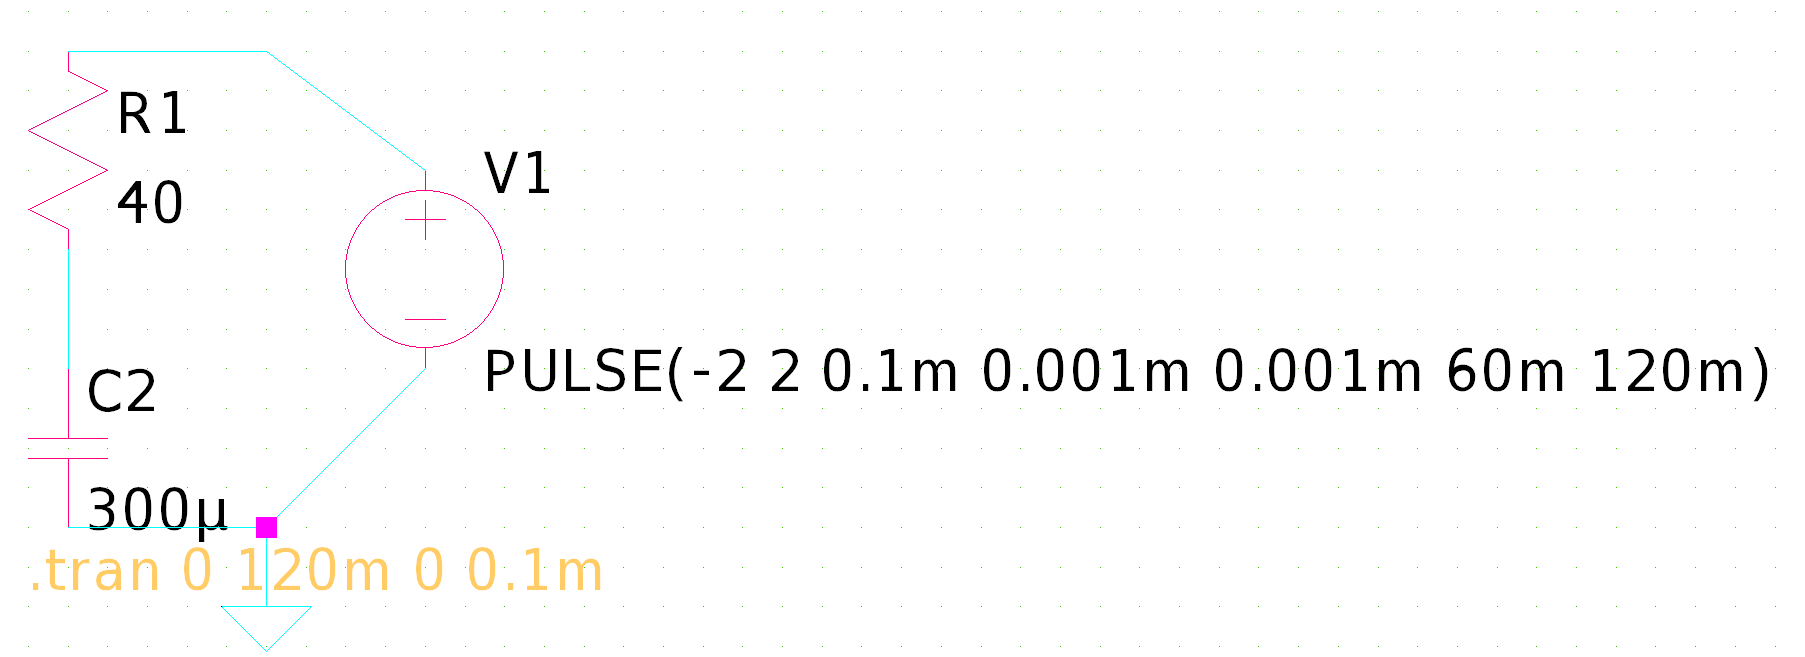
\includegraphics[width=0.6\textwidth]{rc-schema.png} % Make sure the path to the image is correct
% 	\caption{Схема замещения источника электрической энергии в LTspice.}
% \end{figure}

\subsubsection{Расчётные формулы и расчёты}

\subsubsection{Графики переходных процессов}

\subsubsection{Таблица результатов 4.2}

\subsection{Исследование RL-цепи}

\subsubsection{Схема исследуемой цепи}
На рисунке 1.1 представлена схема замещения источника электрической энергии постоянного тока и нагрузки, созданная в приложении LTspice.

% \begin{figure}[H]
% 	\centering
% 	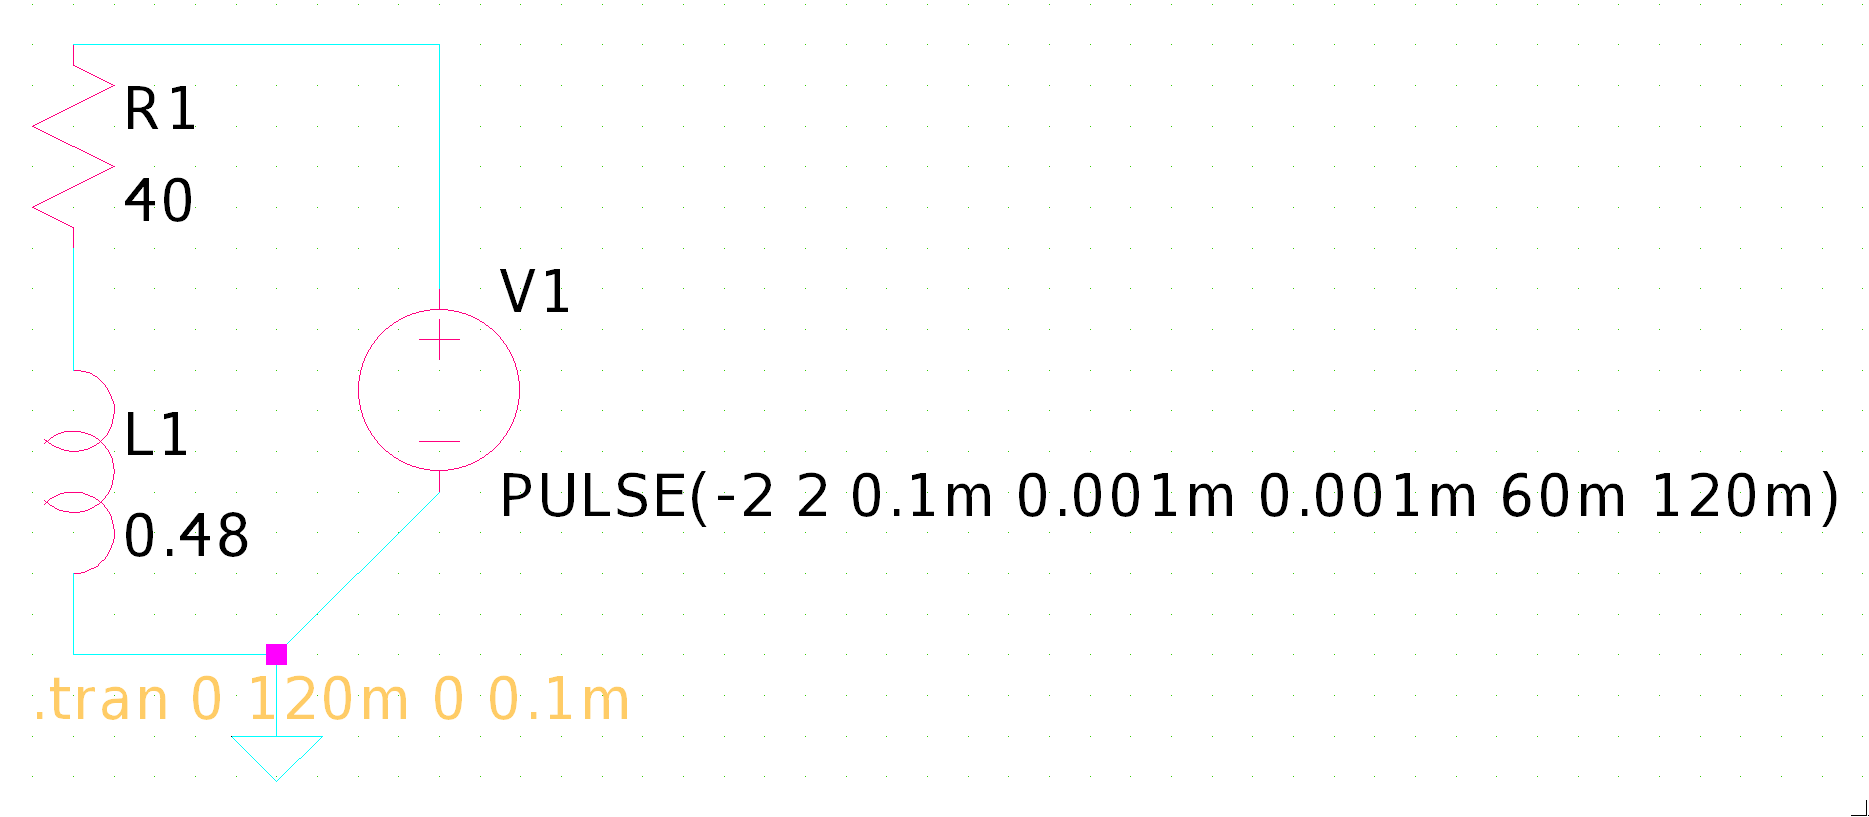
\includegraphics[width=0.6\textwidth]{rl-schema.png} % Make sure the path to the image is correct
% 	\caption{Схема замещения источника электрической энергии в LTspice.}
% \end{figure}

\subsubsection{Расчётные формулы и расчёты}

\subsubsection{Графики переходных процессов}

\subsubsection{Таблица результатов 4.3}

\subsection{Выводы по первой части}
